\PassOptionsToPackage{unicode=true}{hyperref} % options for packages loaded elsewhere
\PassOptionsToPackage{hyphens}{url}
%
\documentclass[]{article}
\usepackage{lmodern}
\usepackage{amssymb,amsmath}
\usepackage{ifxetex,ifluatex}
\usepackage{fixltx2e} % provides \textsubscript
\ifnum 0\ifxetex 1\fi\ifluatex 1\fi=0 % if pdftex
  \usepackage[T1]{fontenc}
  \usepackage[utf8]{inputenc}
  \usepackage{textcomp} % provides euro and other symbols
\else % if luatex or xelatex
  \usepackage{unicode-math}
  \defaultfontfeatures{Ligatures=TeX,Scale=MatchLowercase}
\fi
% use upquote if available, for straight quotes in verbatim environments
\IfFileExists{upquote.sty}{\usepackage{upquote}}{}
% use microtype if available
\IfFileExists{microtype.sty}{%
\usepackage[]{microtype}
\UseMicrotypeSet[protrusion]{basicmath} % disable protrusion for tt fonts
}{}
\IfFileExists{parskip.sty}{%
\usepackage{parskip}
}{% else
\setlength{\parindent}{0pt}
\setlength{\parskip}{6pt plus 2pt minus 1pt}
}
\usepackage{hyperref}
\hypersetup{
            pdftitle={Plantilla arc42},
            pdfborder={0 0 0},
            breaklinks=true}
\urlstyle{same}  % don't use monospace font for urls
\usepackage{longtable,booktabs}
% Fix footnotes in tables (requires footnote package)
\IfFileExists{footnote.sty}{\usepackage{footnote}\makesavenoteenv{longtable}}{}
\usepackage{graphicx,grffile}
\makeatletter
\def\maxwidth{\ifdim\Gin@nat@width>\linewidth\linewidth\else\Gin@nat@width\fi}
\def\maxheight{\ifdim\Gin@nat@height>\textheight\textheight\else\Gin@nat@height\fi}
\makeatother
% Scale images if necessary, so that they will not overflow the page
% margins by default, and it is still possible to overwrite the defaults
% using explicit options in \includegraphics[width, height, ...]{}
\setkeys{Gin}{width=\maxwidth,height=\maxheight,keepaspectratio}
\setlength{\emergencystretch}{3em}  % prevent overfull lines
\providecommand{\tightlist}{%
  \setlength{\itemsep}{0pt}\setlength{\parskip}{0pt}}
\setcounter{secnumdepth}{0}
% Redefines (sub)paragraphs to behave more like sections
\ifx\paragraph\undefined\else
\let\oldparagraph\paragraph
\renewcommand{\paragraph}[1]{\oldparagraph{#1}\mbox{}}
\fi
\ifx\subparagraph\undefined\else
\let\oldsubparagraph\subparagraph
\renewcommand{\subparagraph}[1]{\oldsubparagraph{#1}\mbox{}}
\fi

% set default figure placement to htbp
\makeatletter
\def\fps@figure{htbp}
\makeatother


\title{Plantilla 
\includegraphics{images/arc42-logo.png}}
\date{2018-12-20}

\begin{document}
\maketitle

\section{}

\textbf{Acerca de arc42}

arc42, La plantilla de documentación para arquitectura de sistemas y de
software.

Por Dr. Gernot Starke, Dr. Peter Hruschka y otros contribuyentes.

Revisión de la plantilla: 7.0 ES (basada en asciidoc), Enero 2017

© Reconocemos que este documento utiliza material de la plantilla de
arquitectura arc 42, \url{http://www.arc42.de}. Creada por Dr. Peter
Hruschka y Dr. Gernot Starke.

\begin{quote}
\textbf{Note}

La versión de esta plantilla contiene textos de ayuda y explicación Se
utiliza para familiarizarse con arc42 y comprender sus conceptos. Para
la documentación de su propio sistema puede utilizar la version
\emph{plain}.
\end{quote}

\hypertarget{section-introduction-and-goals}{%
\section{Introducción y Metas}\label{section-introduction-and-goals}}

Describe los requerimientos relevantes y las directrices que los
arquitectos de software y el equipo de desarrollo deben considerar.
Entre estas se incluyen:

\begin{itemize}
\item
  Objetivos empresariales subyacentes, características esenciales y
  requerimientos funcionales para el sistema
\item
  Metas de calidad para la arquitectura
\item
  Las partes interesadas pertinentes y sus expectativas
\end{itemize}

\hypertarget{_vista_de_requerimientos}{%
\subsection{Vista de Requerimientos}\label{_vista_de_requerimientos}}

\textbf{Contenido.}

Descripción corta de los requerimientos funcionales, motivaciones,
extracto (o resumen) de los requerimientos. Ligar a los documentos de
requerimientos determinados (Con número de versión e información de
donde encontrarla).

\textbf{Motivación.}

Desde el punto de vista de los usuarios finales un sistema es creado o
modificado para mejorar el soporte a una actividad de negocio o
incrementar su calidad

\textbf{Forma.}

Descripción corta textual, probablemente en un formato de caso de uso
tabular. Si existen documentos de requerimientos esta vista debe referir
a dichos requerimientos

Mantenga estos extractos tan cortos como sea posible. Encuentre el
balance entre la legibilidad y la redundancia de este documento respecto
a los documentos de requerimientos que se encuentren relacionados.

\hypertarget{_metas_de_calidad}{%
\subsection{Metas de Calidad}\label{_metas_de_calidad}}

\textbf{Contenido.}

Las tres metas de calidad principales (o hasta cinco) cuyo cumplimiento
sea de la mayor importancia para las principales partes interesadas. Nos
referimos a las metas de calidad para la arquitectura. No confundir con
las metas del proyecto. No necesariamente son idénticas.

\textbf{Motivación.}

Debe conocer las metas de calidad de las partes interesadas más
importantes, ya que ellos influenciarán las decisiones arquitectónicas
principales. Asegúrese de ser muy concreto con las descripciones,
evitando buzzwords. Si como arquitecto no conoce la calidad de su
trabajo, será juzgado\ldots{}

\textbf{Forma.}

Una tabla con metas de calidad y escenarios concretos, ordenados por
prioridades

\hypertarget{_partes_interesadas_stakeholders}{%
\subsection{Partes interesadas
(Stakeholders)}\label{_partes_interesadas_stakeholders}}

\textbf{Contenido.}

Vista detallada de las partes intersadas del sistema, es decir, toda
persona, rol u organización que:

\begin{itemize}
\item
  Debe conocer la arquitectura
\item
  Debe estar convencida de la arquitectura
\item
  Tiene que trabajar con la arquitectura o con el código
\item
  Necesitan la documentación de la arquitectura para su trabajo
\item
  Intervienen en las decisiones acerca del sistema o su desarrollo
\end{itemize}

\textbf{Motivación.}

Debe conocer a todas las partes involucradas en el desarrollo del
sistema o que son afectadas por el sistema. De otro modo, se topará con
sorpresas desagradables durante el proceso de desarrollo. Estas partes
relacionadas o stakeholders determinarán la extensión y el nivel de
detalle del trabajo y sus resultados

\textbf{Forma.}

Tabla con nombres de los roles, personas, y sus expectativas con
respecto a la arquitectura y su documentación

\begin{longtable}[]{@{}lll@{}}
\toprule
\begin{minipage}[b]{0.18\columnwidth}\raggedright
Rol/Nombre\strut
\end{minipage} & \begin{minipage}[b]{0.37\columnwidth}\raggedright
Contacto\strut
\end{minipage} & \begin{minipage}[b]{0.37\columnwidth}\raggedright
Expectativas\strut
\end{minipage}\tabularnewline
\midrule
\endhead
\begin{minipage}[t]{0.18\columnwidth}\raggedright
\emph{\textless{}Role-1\textgreater{}}\strut
\end{minipage} & \begin{minipage}[t]{0.37\columnwidth}\raggedright
\emph{\textless{}Contact-1\textgreater{}}\strut
\end{minipage} & \begin{minipage}[t]{0.37\columnwidth}\raggedright
\emph{\textless{}Expectation-1\textgreater{}}\strut
\end{minipage}\tabularnewline
\begin{minipage}[t]{0.18\columnwidth}\raggedright
\emph{\textless{}Role-2\textgreater{}}\strut
\end{minipage} & \begin{minipage}[t]{0.37\columnwidth}\raggedright
\emph{\textless{}Contact-2\textgreater{}}\strut
\end{minipage} & \begin{minipage}[t]{0.37\columnwidth}\raggedright
\emph{\textless{}Expectation-2\textgreater{}}\strut
\end{minipage}\tabularnewline
\bottomrule
\end{longtable}

\hypertarget{section-architecture-constraints}{%
\section{Restricciones de la
Arquitectura}\label{section-architecture-constraints}}

\textbf{Contenido.}

Cualquier requerimiento que restrinja a los arquitectos de software en
la libertad de diseño y la toma de decisiones sobre la implementación o
el proceso de desarrollo. Estas restricciones a veces van más allá de
sistemas individuales y son validos para organizaciones y compañías
enteras.

\textbf{Motivación.}

Los arquitectos deben saber exactamente sus libertades respecto a las
decisiones de diseño y en donde deben apegarse a restricciones. Las
restricciones siempre deben ser acatadas, aunque en algunos casos pueden
ser negociables.

\textbf{Forma.}

Tablas de restricciones con sus explicaciones. Si se requiere, se pueden
subdividir en restricciones técnicas, organizacionales y/o políticas y
convenciones (por ejemplo, guías de versionado o programación,
convenciones de documentación o nombrado)

\hypertarget{section-system-scope-and-context}{%
\section{Alcance y Contexto del
Sistema}\label{section-system-scope-and-context}}

\textbf{Contenido.}

El alcance y contexto del sistema - como lo sugiere el nombre - delimita
al sistema (es decir, el alcance) de todos sus socios de comunicación
(Usuarios y sistemas vecinos, es decir, el contexto del sistema). System
scope and context - as the name suggests - delimits your system (i.e.
your scope) from all its communication partners (neighboring systems and
users, i.e. the context of your system). Con ello se especifican las
interfaces externas.

Si es necesario, diferenciar el contexto de negocio (Entradas y salidas
específicas del dominio) del contexto técnico (canales, protocolos,
hardware).

\textbf{Motivación.}

Las interfases de dominio y las interfases técnicas a los socios de
comunicación son de los aspectos más críticos del sistema. Se debe
asegurar el entendimiento de ellos.

\textbf{Forma.}

Varias opciones:

\begin{itemize}
\item
  Diagramas de contexto
\item
  Listas de socios de comunicación y sus interfases.
\end{itemize}

\hypertarget{_contexto_de_negocio}{%
\subsection{Contexto de Negocio}\label{_contexto_de_negocio}}

\textbf{Contenido.}

La especificación de \textbf{todos} los socios de comunicación
(usuarios, sistemas, \ldots{}) con explicaciones de las entradas y
salidas específicas del dominio o interfases. Opcionalmente puede
agregar formatos específicos de dominio o protocolos de comunicación

\textbf{Motivación.}

Todas las partes interesadas deben entender que datos son intercambiados
con el ambiente del sistema.

\textbf{Forma.}

Cualquier forma de diagramas que muestren al sistema como una caja negra
y especifiquen las interfases de dominio a los socios de comunicación.

De manera alternativa (o adicional) se puede utilizar una tabla. El
título de la tabla es el nombre del sistema, las tres columnas contienen
el nombre del socio de comunicación, las entradas y las salidas

\textbf{\textless{}Diagrama o Tabla\textgreater{}}

\textbf{\textless{}optionally: Explanation of external domain
interfaces\textgreater{}}

\hypertarget{_contexto_t_cnico}{%
\subsection{Contexto Técnico}\label{_contexto_t_cnico}}

\textbf{Contenido.}

Las interfases técnicas (medios de transmisión y canales) enlanzando al
sistema con su ambiente. De manera adicional el mapeo de las
entradas/salidas específicas del dominio a los canales, es decir, una
explicación acerca de que entrada/salida utiliza cual canal.

\textbf{Motivación.}

Muchas partes relacionadas realizan decisiones arquitectónicas basadas
en las interfases técnicas entre el sistema y su contexto. Especialmente
los diseñadores de infraestructura o hardware deciden estas interfases
técnicas.

\textbf{Forma.}

Por ejemplo, diagramas UML de despligue describiendo los canales a
sistemas vecinos, junto con una tabla de mapeo mostrando las relaciones
entre los canales y las entradas/salidas.

\textbf{\textless{}Diagrama o Tabla\textgreater{}}

\textbf{\textless{}Opcional: Explicación de las interfases
técnicas\textgreater{}}

\textbf{\textless{}Mapeo de Entrada/Salida a canales\textgreater{}}

\hypertarget{section-solution-strategy}{%
\section{Estrategia de solución}\label{section-solution-strategy}}

\textbf{Contenido.}

Un resumen corto y explicación de las estrategias y decisiones
fundamentales para la solución que le dan forma a la arquitectura del
sistema. Estas incluyen:

\begin{itemize}
\item
  Decisiones tecnológicas
\item
  Decisiones acerca de la descomposición a alto nivel de un sistema, por
  ejemplo, el uso de algún patrón de diseño o de arquitectura.
\item
  Decisiones en como alcanzar metas de calidad claves
\item
  Decisiones organizacionales relevantes, como el seleccionar un proceso
  de desarrollo o delegar ciertas tareas a terceros.
\end{itemize}

\textbf{Motivación.}

Estas decisiones son las piedras angulares de la arquitectura. Son la
base de muchas otras decisiones detalladas o reglas de implementación.

\textbf{Forma.}

Realice la explicación de las deciciones clave de manera breve.

Justifique las decisiones y porque se realizaron de esa manera, basado
en el planteamiento del problema, las metas de calidad y restricciones
clave. Refierase a los detalles en las secciones posteriores.

\hypertarget{section-building-block-view}{%
\section{Vista de Bloques}\label{section-building-block-view}}

\textbf{Contenido.}

La vista de bloques muestra la descomposición estática del sistema en
bloques de construcción (módulos, componentes, subsistemas, clases,
interfases, paquetes, bibliotecas, marcos de desarrollo, capas,
particiones, funciones, macros, operaciones, estructuras de
datos,\ldots{}) así como sus dependencias (relaciones,
asociaciones,\ldots{})

Esta vista es obligatoria para cualquier documentación de arquitectura.
Es la analogía al plano de una casa.

\textbf{Motivación.}

Mantener una visión general de su código fuente haciendo su estructura
comprensible de manera abstracta.

Esto permite comunicar a las partes interesades en un nivel abstracto
sin entrar en detalles de implementación.

\textbf{Forma.}

La vista de bloques comprende una colección jerárquica de cajas negras y
cajas blancas (ver figura de abajo) y sus descripciones.

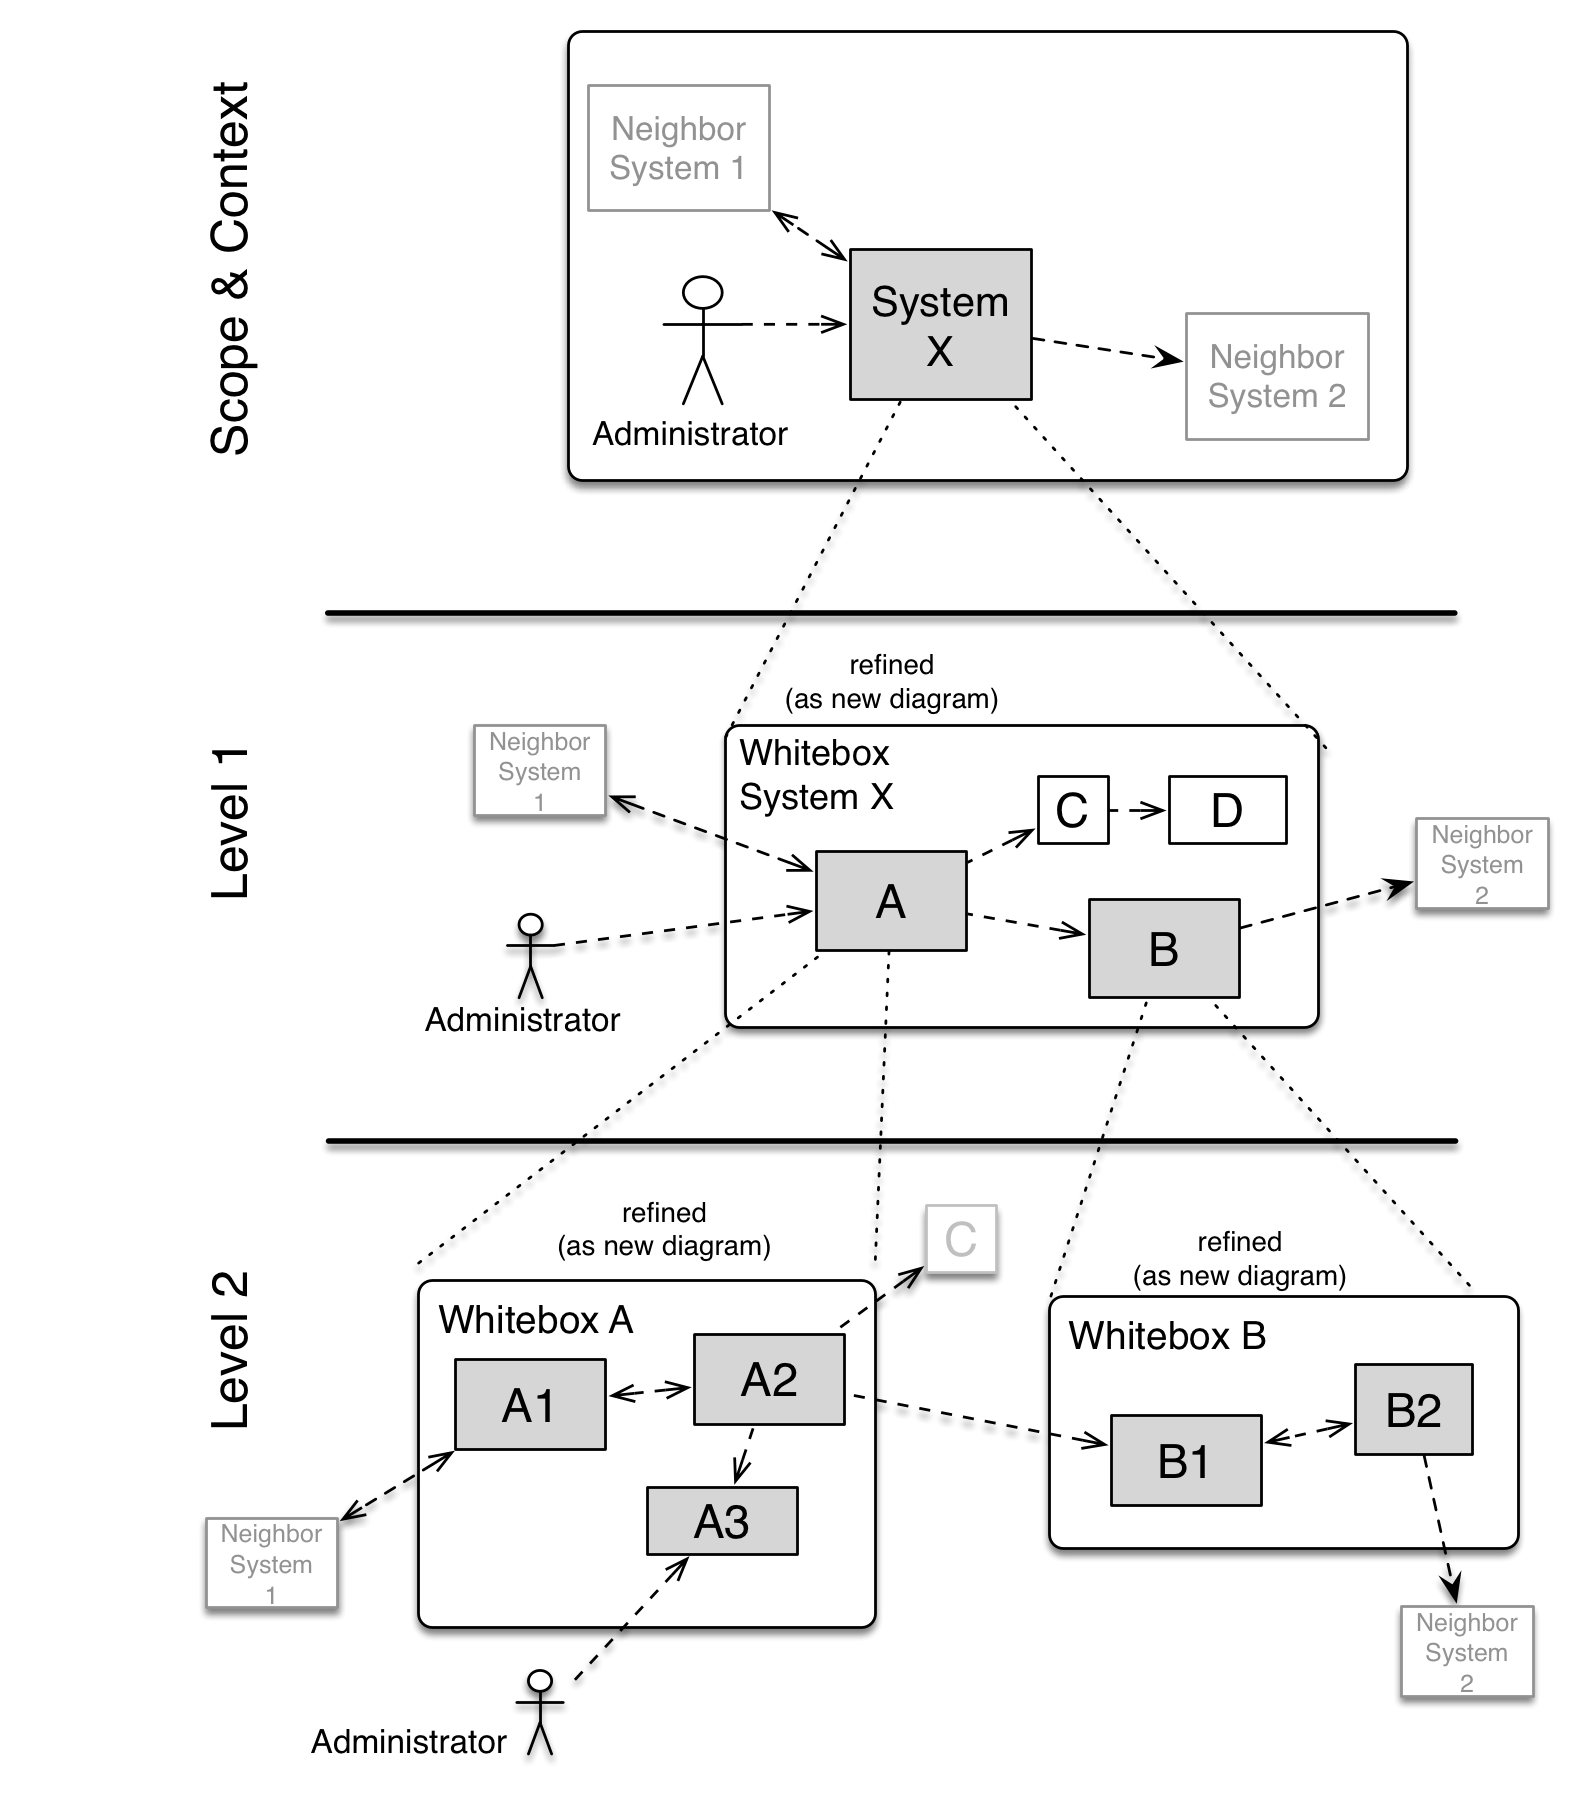
\includegraphics{images/05_building_blocks-ES.png}

\textbf{Nivel 1} comprende la descripción de Caja Blanca del sistema en
general junto con las descripciones de Caja Negra de todos los bloques
contenidos.

\textbf{Nivel 2} hace zoom a los bloques de construcción del Nivel 1.
Entonces contiene la descripción de Caja Blanca de los bloques de
construcción selecionadas del nivel 1,junto con las descripciones de
caja negra de sus bloques de construcción internas.

\textbf{Nivel 3} Hace zoom a los bloques selectos del nivel 2, y así
sucesivamente.

\hypertarget{_sistema_general_de_caja_blanca}{%
\subsection{Sistema General de Caja
Blanca}\label{_sistema_general_de_caja_blanca}}

Aquí se describe la descomposición del sistema en general usando la
siguiente plantilla de caja blanca. Contiene:

\begin{itemize}
\item
  Un diagrama general
\item
  La motivación para la descomposición
\item
  Descripciones de caja negra de los bloques de construcción contenidos.
  Para estos se ofrecen las siguientes alternativas:

  \begin{itemize}
  \item
    Usar \emph{una} tabla para una revisión pragmática y corta de todos
    los bloques de construcción contenidos y sus interfaces
  \item
    Usar una lista de descripciones de caja negra de los bloques de
    construcción acorde a la plantilla de caja negra (ver abajo).
    Dependiendo de la herramienta utilizada, esta lista podría constar
    de sub-capítulos (en archivos de texto), sub-páginas (en un wiki) o
    elementos anidados (en una herramienta de modelado).
  \end{itemize}
\item
  (opcional:) Interfases importantes, que no están explicadas en las
  plantillas de caja negra de un bloque de construcción, pero que son
  muy importantes para entender la caja blanca. En el peor de los casos
  se deberá especificar y desribir la sintaxis, semántica, protocolos,
  manejo de errores, restricciones, versiones, calidades,
  compatibilidades necesarias, entre otras. En el mejor de los casos
  bastará con ejemplos o la firma de los mismos.
\end{itemize}

\emph{\textbf{\textless{}Diagrama general\textgreater{}}}

\begin{description}
\item[Motivación]
\emph{\textless{}Explicación en texto\textgreater{}}
\item[Bloques de construcción contenidos]
\emph{\textless{}Desripción de los bloques de construcción contenidos
(Cajas negras)\textgreater{}}
\item[Interfases importantes]
\emph{\textless{}Descripción de las interfases
importantes\textgreater{}}
\end{description}

Inserte las explicaciones de las cajas negras del nivel 1:

Si usa la forma tabular solo describa las cajas negras con nombre y
responsabilidad acorde al siguiente esquema:

\begin{longtable}[]{@{}ll@{}}
\toprule
\begin{minipage}[b]{0.31\columnwidth}\raggedright
\textbf{Nombre}\strut
\end{minipage} & \begin{minipage}[b]{0.63\columnwidth}\raggedright
\textbf{Responsabilidad}\strut
\end{minipage}\tabularnewline
\midrule
\endhead
\begin{minipage}[t]{0.31\columnwidth}\raggedright
\emph{\textless{}caja negra 1\textgreater{}}\strut
\end{minipage} & \begin{minipage}[t]{0.63\columnwidth}\raggedright
~\emph{\textless{}Texto\textgreater{}}\strut
\end{minipage}\tabularnewline
\begin{minipage}[t]{0.31\columnwidth}\raggedright
\emph{\textless{}caja negra 2\textgreater{}}\strut
\end{minipage} & \begin{minipage}[t]{0.63\columnwidth}\raggedright
~\emph{\textless{}Texto\textgreater{}}\strut
\end{minipage}\tabularnewline
\bottomrule
\end{longtable}

Si utiliza una lista de descripciones de cajas negras entonces llene una
plantilla de caja negra por cada bloque de construcción importante. El
título es el nombre de la caja negra.

\hypertarget{__caja_negra_1}{%
\subsubsection{\textless{}Caja Negra
1\textgreater{}}\label{__caja_negra_1}}

Aqui se describe la \textless{}caja negra 1\textgreater{} acorde a la
siguiente plantilla:

\begin{itemize}
\item
  Propósito/Responsabilidad
\item
  Interfases, cuando no son extraídas como párrafos separados. Estas
  interfases pueden incluir características de calidad y rendimiento.
\item
  (Opcional) Características de Calidad / Rendimiento de la caja negra,
  por ejemplo, disponibilidad, comportamiento en ejecución, \ldots{}
\item
  (Opcional) Ubicación archivo/directorio
\item
  (Opcional) Requerimientos satisfechos (si se necesita contar con la
  trazabilidad a los requerimientos).
\item
  (Opcional) Incidentes/problemas/riesgos abiertos
\end{itemize}

\emph{\textless{}Propósito/Responsabilidad\textgreater{}}

\emph{\textless{}Interfase(s)\textgreater{}}

\emph{\textless{}(Opcional) Características de
Calidad/Performance\textgreater{}}

\emph{\textless{}(Opcional) Ubicación Archivo/Directorio\textgreater{}}

\emph{\textless{}(Opcional) Requerimientos Satisfechos\textgreater{}}

\emph{\textless{}(Opcional) Riesgos/Problemas/Incidentes
Abiertos\textgreater{}}

\hypertarget{__caja_negra_2}{%
\subsubsection{\textless{}Caja Negra
2\textgreater{}}\label{__caja_negra_2}}

\emph{\textless{}plantilla de caja negra\textgreater{}}

\hypertarget{__caja_negra_n}{%
\subsubsection{\textless{}Caja Negra
N\textgreater{}}\label{__caja_negra_n}}

\emph{\textless{}Plantilla de caja negra\textgreater{}}

\hypertarget{__interfase_1}{%
\subsubsection{\textless{}Interfase
1\textgreater{}}\label{__interfase_1}}

\ldots{}

\hypertarget{__interfase_m}{%
\subsubsection{\textless{}Interfase
m\textgreater{}}\label{__interfase_m}}

\hypertarget{_nivel_2}{%
\subsection{Nivel 2}\label{_nivel_2}}

Aquí se especifica la estructura interna de (algunos) bloques de
construcción del nivel 1 como cajas blancas.

Debe decidir cuales bloques de construcción del sistema son lo
suficientemente importantes para justificar una descripción detallada.
Prefiera la relevancia sobre la completitud. Especifique bloques de
construcción importantes, sorprendentes, riesgosos, complejos o
volátiles. Deje fuera las partes normales, simples, estándares o
aburridas del sistema.

\hypertarget{_caja_blanca_emphasis_bloque_de_construcci_n_1_emphasis}{%
\subsubsection{\texorpdfstring{Caja Blanca \emph{\textless{}bloque de
construcción
1\textgreater{}}}{Caja Blanca \textless{}bloque de construcción 1\textgreater{}}}\label{_caja_blanca_emphasis_bloque_de_construcci_n_1_emphasis}}

\ldots{}Describe la estructura interna de \emph{bloque de construcción
1}.

\emph{\textless{}plantilla de caja blanca\textgreater{}}

\hypertarget{_caja_blanca_emphasis_bloque_de_construcci_n_2_emphasis}{%
\subsubsection{\texorpdfstring{Caja Blanca \emph{\textless{}bloque de
construcción
2\textgreater{}}}{Caja Blanca \textless{}bloque de construcción 2\textgreater{}}}\label{_caja_blanca_emphasis_bloque_de_construcci_n_2_emphasis}}

\emph{\textless{}plantilla de caja blanca\textgreater{}}

\ldots{}

\hypertarget{_caja_blanca_emphasis_bloque_de_construcci_n_m_emphasis}{%
\subsubsection{\texorpdfstring{Caja Blanca \emph{\textless{}bloque de
construcción
m\textgreater{}}}{Caja Blanca \textless{}bloque de construcción m\textgreater{}}}\label{_caja_blanca_emphasis_bloque_de_construcci_n_m_emphasis}}

\emph{\textless{}plantilla de caja blanca\textgreater{}}

\hypertarget{_nivel_3}{%
\subsection{Nivel 3}\label{_nivel_3}}

Aqui se especifica la estructura interna de (algunos) de los bloques de
construcción del nivel 2 como cajas blancas.

Cuando la arquitectura requiera más niveles detallados copiar esta
sección para niveles adicionales.

\hypertarget{_caja_blanca_bloque_de_construcci_n_x_1}{%
\subsubsection{Caja Blanca \textless{}\_bloque de construcción
x.1\_\textgreater{}}\label{_caja_blanca_bloque_de_construcci_n_x_1}}

Especifica la estructura interna de \emph{bloque de construcción x.1}.

\emph{\textless{}plantilla de caja blanca\textgreater{}}

\hypertarget{_caja_blanca_bloque_de_construcci_n_x_2}{%
\subsubsection{Caja Blanca \textless{}\_bloque de construcción
x.2\_\textgreater{}}\label{_caja_blanca_bloque_de_construcci_n_x_2}}

\emph{\textless{}plantilla de caja blanca\textgreater{}}

\hypertarget{_caja_blanca_bloque_de_construcci_n_y_1}{%
\subsubsection{Caja Blanca \textless{}\_bloque de construcción
y.1\_\textgreater{}}\label{_caja_blanca_bloque_de_construcci_n_y_1}}

\emph{\textless{}plantilla de caja blanca\textgreater{}}

\hypertarget{section-runtime-view}{%
\section{Vista de Ejecución}\label{section-runtime-view}}

\textbf{Contenido.}

La vista de ejecución describe el comportamiento concreto y la
interacción de los bloques de construcción del sistema en forma de
escenarios en las siguientes áreas:

\begin{itemize}
\item
  Casos de uso o características importantes: ¿Cómo los ejecutan los
  bloques de construcción?
\item
  Interacciones en interfases externas críticas: ¿Cómo cooperan los
  bloques de construcción con los usuarios y sistemas vecinos?
\item
  Administración y operación: Carga, inicialización, detención.
\item
  Escenarios de error y excepción.
\end{itemize}

Observación: El criterio principal para la elección de los escenarios
posibles (flujos de trabajo, secuencias) es su \textbf{relevancia
arquitectónica}. \textbf{No} es importante describir un gran número de
escenarios. Se debe documentar una selección representativa.

\textbf{Motivación.}

Debe entenderse como las instancias de los bloques de construcción del
sistema realizan su trabajo y se comunican en tiempo de ejecución. Deben
capturarse principalmente los escenarios que comuniquen a las partes
relacionadas que tengan problemas para comprender los modelos estáticos
en la documentación (Vista de Bloques de Construcción, Vista de
Despliegue).

\textbf{Forma.}

Hay muchas notaciones para describir los escenarios, por ejemplo: *
Lista numerada de pasos (en lenguaje natural). * Diagramas de flujo o de
actividades * Diagramas de secuencia * BPMN o EPCs (Cadenas de procesos
de eventos) * Máquinas de estado * \ldots{}.

\hypertarget{__escenario_de_ejecuci_n_1}{%
\subsection{\textless{}Escenario de ejecución
1\textgreater{}}\label{__escenario_de_ejecuci_n_1}}

\begin{itemize}
\item
  \emph{\textless{}Inserte un diagrama de ejecución o la descripción del
  escenario\textgreater{}}
\item
  \emph{\textless{}Inserte la descripción de aspectos notables de las
  interacciones entre los bloques de construcción mostrados en este
  diagrama.\textgreater{}}
\end{itemize}

\hypertarget{__escenario_de_ejecuci_n_2}{%
\subsection{\textless{}Escenario de ejecución
2\textgreater{}}\label{__escenario_de_ejecuci_n_2}}

\hypertarget{_}{%
\subsection{\ldots{}}\label{_}}

\hypertarget{__escenario_de_ejecuci_n_n}{%
\subsection{\textless{}Escenario de ejecución
n\textgreater{}}\label{__escenario_de_ejecuci_n_n}}

\hypertarget{section-deployment-view}{%
\section{Vista de Despliegue}\label{section-deployment-view}}

\textbf{Contenido.}

La vista de despliegue describe:

\begin{enumerate}
\def\labelenumi{\arabic{enumi}.}
\item
  La infraestructura técnica usada para ejecutar el sistema, con
  elementos de infraestructura como locaciones geográficas, ambientes,
  computadoras, procesadores, canales y topologías de red así como otros
  elementos de infraestructura.
\item
  El mapeo de los bloques de construcción (software) en dichos elementos
  de infraestructura.
\end{enumerate}

Comúnmente los sistemas son ejecutados en diferentes ambientes, por
ejemplo, ambiente de desarrollo, de pruebas, de producción. En dichos
casos deberían documentarse todos los ambientes relevantes.

Deberá documentarse la vista de despliegue de manera especial cuando el
software se ejecute como un sistema distribuido con mas de una
computadora, procesador, servidor o contenedor o cuando se diseñen los
procesadores y chips de hardware propios.

Desde una perspectiva de software es suficiente con capturar los
elementos de la infraestructura necesarios para mostrar el despliegue de
los bloques de construcción. Los arquitectos de hardware pueden ir más
alla y describir la infraestructura a cualquier nivel de detalle que
requieran.

\textbf{Motivación.}

El software no corre sin haardware. El hardware subyacente puede
influenciar el sistema o algunos conceptos entrecruzados. Por ende, es
necesario conocer la infraestructura.

\textbf{Forma.}

Quizá el más alto nivel de diagrama de despliegue esté contenido en la
sección 3.2. como contexto técnico con la propia infraestructura como
UNA caja negra. En esta sección se deberá realizar un acercamiento a
ésta caja negra utilizando diagramas de despliegue adicionales:

\begin{itemize}
\item
  UML provee diagramas de despliegue para expresar la vista. Uselos,
  probablemente con diagramas anidados.
\item
  Cuando las partes relacionadas de Hardware prefieran otro tipo de
  diagramas además de los diagramas de despliegue, permítales usar
  cualquier tipo que permita mostrar los nodos y canales de la
  infraestructura.
\end{itemize}

\hypertarget{_nivel_de_infraestructura_1}{%
\subsection{Nivel de infraestructura
1}\label{_nivel_de_infraestructura_1}}

Describa (Usualmente en una combinación de diagramas, tablas y texto):

\begin{itemize}
\item
  La distribución del sistema en múltiples ubicaciones, ambientes,
  computadoras, procesadores, \ldots{} así como las conexiones físicas
  entre ellos
\item
  La motivación o justificación de importancia para la estructura de
  despliegue
\item
  Características de Calidad y/o rendimiento de la infraestructura
\item
  El mapeo de los artefactos de software a los elementos de la
  infraestructura.
\end{itemize}

Para múltiples ambientes o despliegues alternativos copie esta sección
para todos los ambientes relevantes.

\emph{\textbf{\textless{}Diagrama General\textgreater{}}}

\begin{description}
\item[Motivación]
\emph{\textless{}Explicación en forma textual\textgreater{}}
\item[Características de Calidad/Rendimiento]
\emph{\textless{}Explicación en forma textual\textgreater{}}

\begin{description}
\item[Mapeo de los Bloques de Construcción a Infraestructura]
\emph{\textless{}Descripción del mapeo\textgreater{}}
\end{description}
\end{description}

\hypertarget{_nivel_de_infraestructura_2}{%
\subsection{Nivel de Infraestructura
2}\label{_nivel_de_infraestructura_2}}

Aquí puede incluir la estructura interna de (algunos) elementos de
infraestructura del nivel 1.

Copie la estructura del nivel 1 para cada elemento elegido.

\hypertarget{__emphasis_elemento_de_infraestructura_1_emphasis}{%
\subsubsection{\texorpdfstring{\emph{\textless{}Elemento de
Infraestructura
1\textgreater{}}}{\textless{}Elemento de Infraestructura 1\textgreater{}}}\label{__emphasis_elemento_de_infraestructura_1_emphasis}}

\emph{\textless{}diagrama + explicación\textgreater{}}

\hypertarget{__emphasis_elemento_de_infraestructura_2_emphasis}{%
\subsubsection{\texorpdfstring{\emph{\textless{}Elemento de
Infraestructura
2\textgreater{}}}{\textless{}Elemento de Infraestructura 2\textgreater{}}}\label{__emphasis_elemento_de_infraestructura_2_emphasis}}

\emph{\textless{}diagrama + explicación\textgreater{}}

\ldots{}

\hypertarget{__emphasis_elemento_de_infraestructura_n_emphasis}{%
\subsubsection{\texorpdfstring{\emph{\textless{}Elemento de
Infraestructura
n\textgreater{}}}{\textless{}Elemento de Infraestructura n\textgreater{}}}\label{__emphasis_elemento_de_infraestructura_n_emphasis}}

\emph{\textless{}diagrama + explicación\textgreater{}}

\hypertarget{section-concepts}{%
\section{Conceptos Transversales
(Cross-cutting)}\label{section-concepts}}

\textbf{Contenido.}

Esta sección describe de manera general, las principales ideas de
solución y regulación que son relevantes en multiples partes (→
cross-cutting/transversales) del sistema. Dichos conceptos están
relacionados usualmente a múltiples bloques de construcción. Pueden
incluir diversos temas, tales como:

\begin{itemize}
\item
  Modelos de dominio
\item
  Patrones de arquitectura o patrones de diseño
\item
  Reglas de uso para alguna tecnología específica.
\item
  Decisiones técnicas principales o generales
\item
  Reglas de implementación
\end{itemize}

\textbf{Motivación.}

Conceptos que forman la base para la \emph{integridad conceptual}
(consistencia, homogeneidad) de la arquitectura. Entonces, son una
contribución importante para alcanzar la calidad interna del sistema.

Algunos de estos conceptos no pueden ser asignados a bloques de
construcción individuales (por ejemplo seguridad). Este es el lugar en
la plantilla provisto para una especificación cohesiva de dichos
conceptos.

\textbf{Forma.}

La forma puede ser variada:

\begin{itemize}
\item
  Papeles conceptuales con cualquier tipo de estructura
\item
  Modelo transversal (cross-cutting) de fragmentos o escenarios usando
  notación de las vistas arquitectónicas
\item
  Implementaciones de muestra, especialmente para conceptos técnicos.
\item
  Referencias a uso típico en frameworks estándar (por ejemplo, el uso
  de Hibernate para mapeo Objeto/Relacional) The form can be varied:
\end{itemize}

\textbf{Estructura.}

La estructura potencial (pero no obligatoria) para esta sección podría
ser:

\begin{itemize}
\item
  Conceptos de dominio
\item
  Conceptos de experiencia de usuario (UX)
\item
  Conceptos de seguridad
\item
  Patrones de diseño y arquitectura * A potential (but not mandatory)
  structure for this section could be:
\item
  Domain concepts
\item
  User Experience concepts (UX)
\item
  Safety and security concepts
\item
  Architecture and design patterns
\item
  "Bajo el capó"
\item
  Conceptos de desarrollo
\item
  Conceptos de operación
\end{itemize}

Nota: Puede ser difícil asignar conceptos individuales a un tema
específico de la lista

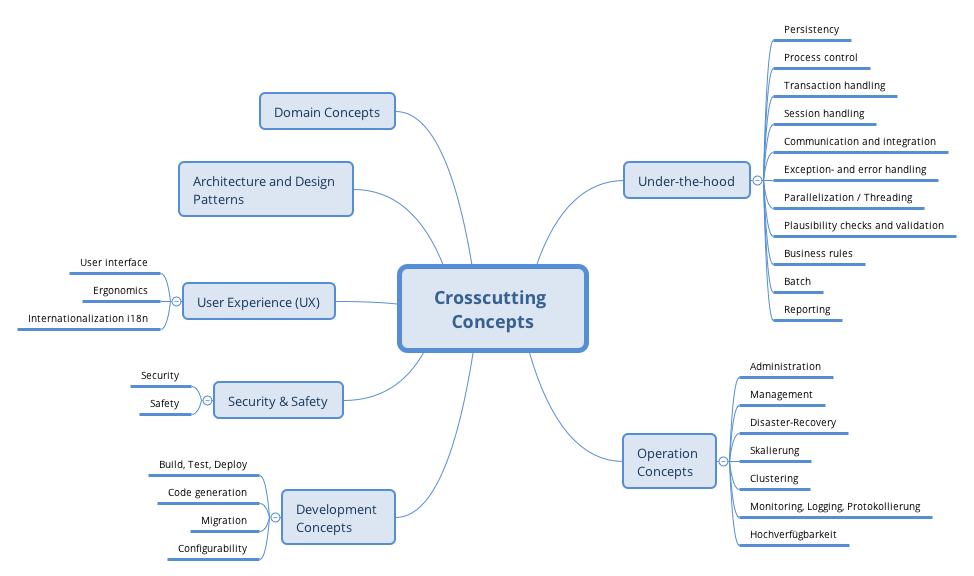
\includegraphics{images/08-Crosscutting-Concepts-Structure-ES.png}

\hypertarget{__emphasis_concepto_1_emphasis}{%
\subsection{\texorpdfstring{\emph{\textless{}Concepto
1\textgreater{}}}{\textless{}Concepto 1\textgreater{}}}\label{__emphasis_concepto_1_emphasis}}

\emph{\textless{}explicación\textgreater{}}

\hypertarget{__emphasis_concepto_2_emphasis}{%
\subsection{\texorpdfstring{\emph{\textless{}Concepto
2\textgreater{}}}{\textless{}Concepto 2\textgreater{}}}\label{__emphasis_concepto_2_emphasis}}

\emph{\textless{}explicación\textgreater{}}

\ldots{}

\hypertarget{__emphasis_concepto_n_emphasis}{%
\subsection{\texorpdfstring{\emph{\textless{}Concepto
n\textgreater{}}}{\textless{}Concepto n\textgreater{}}}\label{__emphasis_concepto_n_emphasis}}

\emph{\textless{}explicación\textgreater{}}

\hypertarget{section-design-decisions}{%
\section{Decisiones de Diseño}\label{section-design-decisions}}

\textbf{Contenido.}

Decisiones arquitectónicas importantes, costosas, a larga escala o
riesgosas incluyendo sus razonamientos. Con "Decisiones" nos referimos a
la elección de una alternativa basada en cierto criterio.

Se debe usar el juicio para decidir si una decisión arquitectónica debe
ser documentada en esta sección central o si sería preferible
documentarla localmente (Por ejemplo, dentro de una plantilla de caja
blanca de un bloque de construcción).

Evite la redundancia. Tomar de referencia la sección 4, donde ya se
capturaron las decisiones más importantes para la arquitectura.

\textbf{Motivación.}

Las partes relacionadas del sistema deben comprender y trazar las
decisiones.

\textbf{Forma.}

Varias opciones:

\begin{itemize}
\item
  Lista o tabla, ordenada por importancia y consecuencias o:
\item
  Mayor detalle en secciones separadas por cada sección.
\item
  Registro de Decisiones de Arquitectura (ADR por sus siglas en inglés)
  para cada decisión importante.
\end{itemize}

\hypertarget{section-quality-scenarios}{%
\section{Requerimientos de Calidad}\label{section-quality-scenarios}}

\textbf{Contenido.}

Esta sección describe todos los requerimientos de calidad como un árbol
de calidad con escenarios. Los más importantes ya han sido descritos en
la sección 1.2 (Metas de Calidad).

Aquí se capturan los requerimientos de calidad con menor prioridad, que
no crearán altos riesgos en caso de que no sean cubiertos con totalidad.

\textbf{Motivación.}

Dado que los requerimientos de calidad tendrán mucha influencia en las
decisiones arquitectónicas deben tomarse en cuenta los elementos
importantes para las partes relacionadas que sean concretas y medibles.

\hypertarget{__rbol_de_calidad}{%
\subsection{Árbol de Calidad}\label{__rbol_de_calidad}}

\textbf{Contenido.}

El árbol de calidad (Definido en ATAM - Método de análisis de
compensación de arquitectura por sus silas en inglés) con escenarios de
calidad/evaluación como hojas.

\textbf{Motivación.}

La estructura de árbol con prioridades provee un vistazo general para un
gran número de requerimientos de calidad.

\textbf{Forma.}

El árbol de calidad es un vistazo a alto nivel de las metas de calidad y
requerimientos:

\begin{itemize}
\item
  Un refinamiento del término de "calidad" a manera de árbol. Utilice
  "calidad" o "utilidad" como raíz.
\item
  Un mapa mental con categorías de calidad como ramas principales
\end{itemize}

En cualquier caso incluya ligas a los escenarios de las siguientes
secciones.

\hypertarget{_escenarios_de_calidad}{%
\subsection{Escenarios de calidad}\label{_escenarios_de_calidad}}

\textbf{Contenido.}

Concretización de requerimientos de calidad (que pueden ser vagos o
implícitos) utilizando escenarios de calidad.

Estos escenarios describen lo que debería pasar cuando un estímulo llega
al sistema.

Para los arquitectos, son importantes dos tipos de escenarios:

\begin{itemize}
\item
  Escenarios de uso (también llamados escenarios de aplicación o
  escenarios de caso de uso), que describen la reacción en tiempo de
  ejecución de un sistema a un determinado estímulo. Esto incluye
  también escenarios que describen la eficiencia o el rendimiento del
  sistema. Por ejemplo: El sistema reacciona a la petición de un usuario
  en un segundo.
\item
  Escenarios de cambios, describen la modificación del sistema a su
  ambiente inmediato. Por ejemplo: Cuando se implementa funcionalidad
  adicional o requerimietnos para el cambio de un atributo de calidad.
\end{itemize}

\textbf{Motivación.}

Los escenarios crean requerimientos de calidad concretos y permiten
medirlos de manera mas sencilla o decidir si han sido cumplidos.

Cuando se requiere evaluar la arquitectura utilizando métodos como ATAM
se necesitan describir las metas de calidad (de la sección 1.2) de
manera más precisa hasta un nivel de escenarios que pueden ser
discutidos y evaluados.

\textbf{Forma.}

Texto en forma libre o tabular.

\hypertarget{section-technical-risks}{%
\section{Riesgos y deuda técnica}\label{section-technical-risks}}

\textbf{Contenido.}

Una lista de los riesgos técnicos o deuda técnica identificada, ordenada
por prioridad.

\textbf{Motivación.}

"El manejo de riesgos es administración de proyectos para gente adulta"
(Tim Lister, Atlantic Systems Guild.)

Esto debiera ser el lema para la detección sistemática y la evaluación
de riesgos y deuda técnica en la arquitectura, que será requerida por
las partes relacionadas administrativas (por ejemplo, administradores de
proyectoes, propietarios de producto) como parte de la planeación y
medición de riesgos en general.

\textbf{Forma.}

Lista de riesgos y/o deuda técnica, que podría incluir una medidas
sugeridas para minimizar, mitigar o evitar riesgos o reducir la deuda
técnica.

\hypertarget{section-glossary}{%
\section{Glosario}\label{section-glossary}}

\textbf{Contenido.}

Los términos técnicos y de dominio más importantes que serán utilizados
por las partes relacionadas al discutir el sistema.

También se puede usar el glosario como fuente para traducciones si se
trabaja en equipos multi-lenguaje.

\textbf{Motivación.}

Deberían definirse claramente los términos, para que todas las partes
relacionadas:

\begin{itemize}
\item
  Tengan un entendimiento idéntico de dichos términos
\item
  No usen sinónimos y homónimos
\end{itemize}

\textbf{Forma.}

Crear una tabla con las columnas \textless{}Término\textgreater{} y
\textless{}Definición\textgreater{}.

Se pueden agregar más columnas en caso de que se requieran traducciones.

\begin{longtable}[]{@{}ll@{}}
\toprule
\begin{minipage}[b]{0.47\columnwidth}\raggedright
Término\strut
\end{minipage} & \begin{minipage}[b]{0.47\columnwidth}\raggedright
Definición\strut
\end{minipage}\tabularnewline
\midrule
\endhead
\begin{minipage}[t]{0.47\columnwidth}\raggedright
\textless{}Término-1\textgreater{}\strut
\end{minipage} & \begin{minipage}[t]{0.47\columnwidth}\raggedright
\textless{}definicion-1\textgreater{}\strut
\end{minipage}\tabularnewline
\begin{minipage}[t]{0.47\columnwidth}\raggedright
\textless{}Término-2\textgreater{}\strut
\end{minipage} & \begin{minipage}[t]{0.47\columnwidth}\raggedright
\textless{}definicion-2\textgreater{}\strut
\end{minipage}\tabularnewline
\bottomrule
\end{longtable}

\end{document}
